% !TEX root = mainthesis.tex
%Chapter 6

% Our system is not the only one suffering from this issues; decoherence of quantum systems due to uncontrolled fluctuations of the environment presents fundamental obstacles in quantum science.
\newcommand{\reffig}[1]{Figure~\ref{#1}}
\newcommand{\refeq}[1]{Equation~\ref{#1}}
\externaldocument{Chapter4.tex}

\renewcommand{\thechapter}{6}

\chapter{Synthetic clock transitions through continuous dynamical decoupling}
\label{ch:clock_states}

Most of the experiments techniques described so far have used the hyperfine $\ket{m_F}$ states as effective spins and dressed them with an RF or Raman field. However, due to the linear dependence of their energies with respect to magnetic field, and our lack of control of environmental changes we always had to take special care to stabilize the magnetic field in the lab (see Section~\ref{sec:ptai}). An alternative to doing active magnetic field stabilization is to use clock transitions which are first-order insensitive to changes in magnetic field but unfortunately they are not present in all systems or for arbitrary system parameters. However, under almost all circumstances, clock transitions can be synthesized using dynamical decoupling protocols. These protocols involve driving the system with an external oscillatory field, resulting in a dynamically protected `dressed' system.

The idea of implementing continuous dynamical decoupling (CDD) in the lab came from a theoretical proposal to engineer Rashba type SOC using Raman beams and a strong RF field~\cite{campbell_rashba_2016}, the second being a necessary ingredient for CDD. We initially worked in implementing CDD protocols to create `synthetic clock states' as an intermediate step towards our final goal of engineering Rashba SOC. Just like with Fourier spectroscopy, CDD became a workhorse of the lab both for the stability it provides against environmental fluctuations and because it has given us access to non-zero matrix coupling elements that we otherwise would not have when working with the bare $\ket{m_F}$ states. We have continued to use CDD  not only for engineering Rashba SOC (Chapter~\ref{ch:Rashba}) but also to engineer subwavelength optical lattices\cite{anderson_realization_2019} and Hofstadter~\cite{hofstadter_energy_1976} cylinders (work in preparation). On the theory side, we developed a proposal that uses them as a platform for emulating $\mathcal{PT}$ symmetric Hamiltonians~\cite{trypogeorgos_perpetual_2018}. 

This Chapter discusses the implementation of CDD in the ground $F=1$ hyperfine manifold of ultracold $\Rb87$. First I give a general overview of dynamical decoupling and continuous dynamical decoupling. Then I describe the technical details and characterization of our CDD protocol which produces a protected three-level system of dressed-states and whose Hamiltonian is fully controllable. Finally, I discuss an implementation of concatenated CDD that renders the system first-order insensitive to both magnetic field noise and noise in the control field. This work was published in~\cite{trypogeorgos_synthetic_2018} and was done in parallel with~\cite{anderson_continuously_2018}.

\section{Basic principles of CDD}

Dynamical decoupling (DD) protocols consist in applying an external control Hamiltonian, generally implemented by a series of pulses, which has the effect of canceling out the dynamics that arise from ta quantum system coupling to the environment. DD was first introduced in the context of nuclear magnetic resonance (NMR) with the discovery of spin-echoes~\cite{hahn_spin_1950}, where a single `refocusing' pulse was applied to eliminate dephasing of spins resulting from variations in magnetic field. These ideas were later generalized in~\cite{viola_dynamical_1998} to protect a system from decoherence induced by interactions with a quantum environment. Continuous dynamical decoupling (CDD) relies on the application of time-periodic continuous control fields, rather than a series of pulses. %Unlike conventional dynamical decoupling protocols, CDD does not require any encoding overhead.% or quantum feedback measurements. 

A number of dynamical decoupling protocols, pulsed or continuous, have been shown to isolate quantum systems from low-frequency environmental noise~\cite{cohen_continuous_2017,fanchini_continuously_2007,aharon_fully_2016,biercuk_optimized_2009,cai_robust_2012,bermudez_robust_2012,baumgart_ultrasensitive_2016,kazakov_magic_2015,sarkany_controlling_2014}. Thus far, CDD has inoculated multi-level systems in nitrogen vacancy centers in diamond, nuclear magnetic resonance experiments, and trapped atomic ions~\cite{laucht_dressed_2017,farfurnik_experimental_2017,noguchi_generation_2012,golter_protecting_2014,timoney_quantum_2011,webster_simple_2013,barfuss_strong_2015,rohr_synchronizing_2014}, from spatiotemporal magnetic field fluctuations. 

\section{CDD of a spin-1 system}
\begin{figure}[!!h]
    \centering
    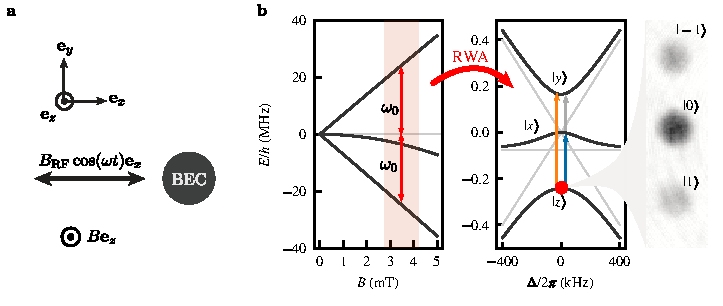
\includegraphics[]{Figures/Chapter6/fig1a.pdf}
    \caption[Implementing CCD.]{{\bf a.} Setup for implementing CCD using a strong RF magnetic field. {\bf b.}  Left: dependence of the $5^2S_{1/2}$, $F=1$ ground state of $\Rb87$ on magnetic field, where the quadratic dependence of the $\ket{m_F=0}$ state's Zeeman shift has been exaggerated so it is visible on the same scale.
    Center: energies of the $\xyz$ eigenstates, for $\Omega/2\pi=\SI{200}{kHz}$ (black curves) and $\Omega=0$ (grey curves).
    Right: TOF absorption image of $\ket{z}$ at $\Delta=0$, showing the constituent $\ket{m_F}$ states.
    }
    \label{fig:1}
\end{figure}

We implemented CDD using a strong RF magnetic field with strength $\Omega$ which linked the three $\ket{m_F}$ states comprising the $F=1$ electronic ground state manifold of $\Rb87$.
The RF field was linearly polarized along ${\bf e}_x$, and had angular frequency $\omega$ close to the Larmor frequency $\omega_0 = g_F \mu_{\rm B} B_0$ from a magnetic field $B_0 {\bf e}_z$; $g_F$ is the Lande $g$-factor and $\mu_{\rm B}$ is the Bohr magneton. Using the rotating frame approximation for the frame rotating at $\omega$ (which is valid for $\omega >>\Omega$), the system is described by
%
\begin{equation}
    \hat{H} = \hbar\Delta\fz+\hbar\epsilon(\fz^2-\hat{\mathbb{1}})+ \hbar\Omega \fx,
    \label{eq:h0}
\end{equation}
with detuning $\Delta=\omega-\omega_0$, quadratic Zeeman shift $\epsilon$, spin-1 angular momentum operators $\hat F_{x,y,z}$, and the identity operator $\hat{\mathbb 1}$.% For a detailed derivation of Equation~\ref{eq:h0} see Section~\ref{seq:rf_coupling}.

\section{The $\xyz$ states}
\label{seq:xyz_states}

The eigenstates of Equation~\ref{eq:h0} correspond to the CDD basis. In this section, I describe their properties and show that their energies are first-order insensitive to magnetic field fluctuations.

\subsection{State decomposition}

We denote the eigenstates of Equation~\ref{eq:h0} by $\ket{x}$, $\ket{y}$ and $\ket{z}$. The CDD states are linear combinations of the $\ket{m_F}$ basis states, and for $\Delta=0$ the (non-normalized) eigenvectors are:
%
\begin{align}
    \ket x =& \ket{-1} - \ket{1}, \nonumber \\
    \ket y =& \ket{-1} -\frac{\epsilon + \tilde\Omega}{\sqrt 2 \Omega} \ket 0 + \ket 1, \\
    \ket z =& \ket{-1} -\frac{\epsilon - \tilde\Omega}{\sqrt 2 \Omega} \ket 0 + \ket 1. \nonumber
\end{align}
%
Figure~{\ref{fig:s1}} shows the normalized full state decomposition as a function of $\Delta$, where it can be seen that the $\xyz$ states adiabatically map to the $\ket{m_F}$ states for $\vert\Delta\vert \gg \Omega$: for positive (negative) detuning $\ket z$ maps to $\ket 1$ ($\ket{-1}$); $\ket y$ maps in the exact opposite way to $\ket z$; and $\ket x$ always maps to $\ket 0$.
\begin{figure*}[ht]
    \centering
    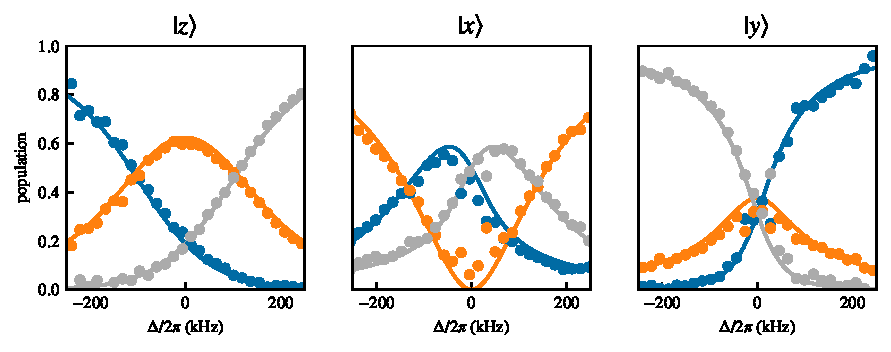
\includegraphics[]{Figures/Chapter6/figS11}
    \caption[State decomposition of the $\xyz$ states]{Decomposition of the $\xyz$ states on the $\ket{m_F}$ basis for $\Omega/2\pi=\SI{145(1)}{kHz}$
    The $\ket{m_F=-1,0,1}$ states correspond to blue, orange, gray respectively.}
    \label{fig:s1}
\end{figure*}

We labeled our dressed states $\xyz$ since for $\Omega\rightarrow 0^+$ and $\Delta=0$, they continuously approach the $\XYZ$ states familiar from quantum chemistry~\cite{cooper_reaching_2013}:
\begin{align}
    \ket X &= \frac{\ket{1} - \ket{-1}}{\sqrt{2}}, \nonumber \\
    \ket Y &= i\frac{\ket{1} + \ket{-1}}{\sqrt{2}}, \\
    \ket Z &= \ket{0}. \nonumber
\end{align}
which transform under the application of the spin-1 operators as $\epsilon_{jkl}\hat F_j \ket k= i\hbar \ket l$, so that a resonant probe field can induce transitions between at least one pair of states, irrespectively of its polarization.

Finally, when $\Omega\to\infty$ they are independent of the driving field amplitude and continuously approach the eigenstates of the $\hat F_x$ operator
\begin{align}
    \ket x &= \ket{1} - \ket{-1}, \nonumber \\
    \ket y &= \ket{1} + \sqrt 2 \ket 0 + \ket{-1}, \\
    \ket z &= \ket{1} - \sqrt 2 \ket 0 + \ket{-1}. \nonumber
\end{align}

\subsection{Energies}

The clock-like nature of these states is determined by their eigenvalues which are even functions with respect to $\Delta$ as can be seen by the leading order expansion of the eigenenergies $E_i=\hbar\omega_i$ for $\Delta\to 0$
\begin{align}
    \omega_x =& -\frac{\epsilon}{\Omega^2} \Delta^2 + \mathcal{O}(\Delta^4), \nonumber \\
    \omega_y =& \frac 12 (-\epsilon + \tilde\Omega) - \frac{(\epsilon + \tilde\Omega)}{-\epsilon^2-4\Omega^2+\epsilon\tilde\Omega} \Delta^2 + \mathcal{O}(\Delta^4), \label{eq:exp} \\
    \omega_z =& \frac 12 (-\epsilon - \tilde\Omega) + \frac{(\epsilon - \tilde\Omega)}{\epsilon^2+4\Omega^2+\epsilon\tilde\Omega} \Delta^2 \nonumber ,
\end{align}
where  we have defined $\tilde\Omega=\sqrt{4\Omega^2+\epsilon^2}$. The energy differences $\hbar\omega_{xy}$, $\hbar\omega_{zy}$ and $\hbar\omega_{zx}$ are only quadratically sensitive to $\Delta$ for $\Delta\ll\Omega$~\footnote{The energies are quadratic in $\Delta$ for $\Delta\ll\Omega$, and linear for $\Delta\gg\Omega$ with a slope of \SI{7}{MHz/mT}.} so that detuning fluctuations $\delta \Delta$ are suppressed to first order, making these a trio of synthetic clock states. The curvatures of $\omega_x$ and $\omega_z$ have the same sign and in principle there is a critical value of $\Omega$ where the quadratic term in transition energy can be made arbitrarily small, making it quartic in $\Delta$. However, this cancellation does not take place when we consider the dependence of $\epsilon$ on $\Delta$ from the Breit-Rabi expression. It is still possible to find an optimal $\Omega$ for which $\omega_{zx}$ depends quartically on $\Delta$, but it does not occur at $\Delta=0$ as is predicted by Equation~\ref{eq:exp} for constant $\epsilon$. 

\subsection{Transition matrix elements}
\label{sec:xyz_matrix_elements}

Unlike the $\ket{m_F}$ basis, an oscillatory magnetic field with the right polarization can drive transitions between all pairs of the $\xyz$ states with non-zero transition matrix elements. The transition matrix elements between the $\xyz$ have a dependence on both $\Omega$ and $\Delta$. For the $\Delta=0$ case they can be read from the representation of the spin-1 matrices in the $\xyz$ basis

\begin{align}
\fx &\rightarrow \begin{pmatrix}
 \frac{2 \Omega }{\tilde{\Omega}} & 0 & -\frac{\epsilon }{\tilde{\Omega}} \nonumber \\
 0 & 0 & 0 \nonumber\\
 -\frac{\epsilon }{\tilde{\Omega}} & 0 & -\frac{2 \Omega }{\tilde{\Omega}} \nonumber\\
\end{pmatrix} \nonumber \\ \nonumber\\
%
\fy &\rightarrow \begin{pmatrix}
 0 & -\frac{i (\tilde{\Omega} -\epsilon )}{\Omega  \sqrt{\frac{(\epsilon -\tilde{\Omega} )^2}{\Omega ^2}+4}} & 0 \nonumber\\
 \frac{i (\tilde{\Omega} -\epsilon )}{\Omega  \sqrt{\frac{(\epsilon -\tilde{\Omega} )^2}{\Omega ^2}+4}} & 0 & -\frac{i (\tilde{\Omega} +\epsilon )}{\Omega 
   \sqrt{\frac{(\tilde{\Omega} +\epsilon )^2}{\Omega ^2}+4}} \nonumber\\
 0 & \frac{i (\tilde{\Omega} +\epsilon )}{\Omega  \sqrt{\frac{(\tilde{\Omega} +\epsilon )^2}{\Omega ^2}+4}} & 0 \\
\end{pmatrix}  \nonumber\\ \nonumber\\
%
\fz &\rightarrow \begin{pmatrix}
 0 & -\frac{\sqrt{\frac{\epsilon }{\tilde{\Omega}}+1}}{\sqrt{2}} & 0 \\
 -\frac{\sqrt{\frac{\epsilon }{\tilde{\Omega}}+1}}{\sqrt{2}} & 0 & -\frac{2}{\sqrt{\frac{\left(\tilde{\Omega}+\epsilon
   \right)^2}{\Omega ^2}+4}} \\
 0 & -\frac{2}{\sqrt{\frac{\left(\tilde{\Omega}+\epsilon \right)^2}{\Omega ^2}+4}} & 0 \\
\end{pmatrix},
\label{eq:matrix_elements}
\end{align}
%
where the states have been ordered by decreasing energy ($\ket{y}$, $\ket{x}$, $\ket{z}$). We therefore see that a term in a Hamiltonian that is proportional to $\fx$ can only drive transitions between $\ket{z}$ and $\ket{y}$ and that a coupling term proportional to $\fy$ and $\fz$ can drive both drive transitions between $\ket{z}$ and $\ket{x}$ or $\ket{x}$ and $\ket{y}$ with different strengths. It can be seen from Equation~\ref{eq:matrix_elements} that when $\Omega$ and $\epsilon$ are comparable in magnitude there exists at least one non-zero transition matrix element for each pair of dressed states and they can all be coupled cyclically.

%  are nonzero and the states can be coupled cyclically.

% For $\Omega \ll \epsilon$ the matrix elements correspond to those of the $\ket{m_F}$ basis and $\langle x \vert \hat F_+ \vert y \rangle = 0$ as expected by angular momentum selection rules. When $\Omega$ and $\epsilon$ are comparable in magnitude al transition matrix elements are nonzero and the states can be coupled cyclically.

% \note{TODO: write matrix elements in dressed basis}
% As $\Omega \gg \epsilon$ the $\ket z$ and $\ket y$ states decouple and the system resembles an `undressed basis' following similar selection rules. \note{I'm not entirely sure how this were computed, I should redo this plots}

% \begin{figure*}[ht]
%     \centering
%     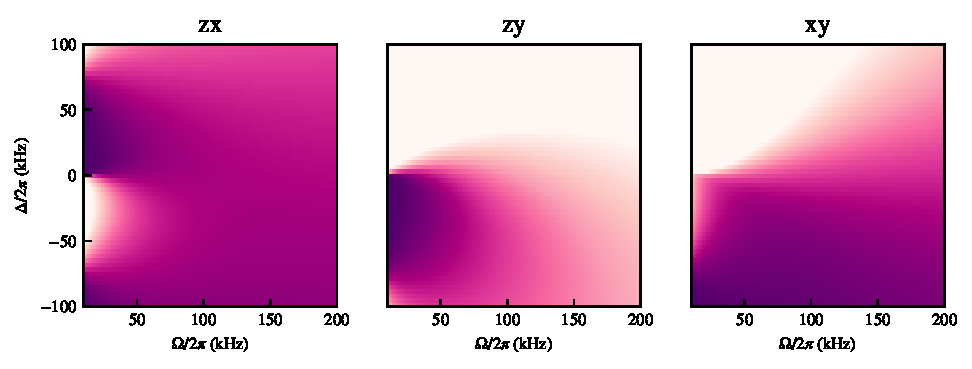
\includegraphics[]{Figures/Chapter6/figS12}
%     \caption[Transition matrix elements over $\Omega$ and $\Delta$.]{Transition matrix elements over $\Omega$ and $\Delta$.
%     There is an assymetry between coupling on the blue and red side of the resonance that corresponds to the counter- and co-rotating terms $\hat F_-$ and $\hat F_+$.}
%     \label{fig:s12}
% \end{figure*}

\section{$\xyz$ state preparation}
\label{sec:xyz_state_preparation}

We implemented CCD to BECs with $N\approx\num{5e4}$ atoms. For all of the experiments described in this Chapter the dipole trap had trapping frequencies of $(f_x,\, f_y,\, f_z) = (42(3),\, 34(2),\, 133(3))$\,Hz. We applied a $B_0 \approx \SI{3.27}{mT}$ bias field that lifted the ground state degeneracy, giving an $\omega_0/2\pi = \SI{22.9}{MHz}$ Larmor frequency, with a quadratic shift $\epsilon/2\pi=\SI{76.4}{kHz}$. We determined that the ambient magnetic field fluctuations were dominated  by contributions from line noise giving an RMS uncertainty $\delta\Delta/2\pi = g_F \mu_{\rm B}\delta B/h=\SI{0.67(3)}{kHz}$.

The state preparation consisted of two stages of ARP. On the first stage we followed the usual protocol described in Section~\ref{sec:arp} to prepare the BEC in any of the $\ket{m_F = 0,-1,1}$ states. On the second stage, we adiabatically transformed the $\ket{m_F}$ states into the $\xyz$ states. We started with the bias field far from resonance ($\Delta(t=0)/2\pi \approx -\SI{450}{kHz}$) and with all coupling fields off. Then we ramped on $\Omega$ in a two-step process. We first ramped from $\Omega=0$ to an intermediate value $\Omega_{\rm mid}$, approximately half its final value in \SI{1}{ms}. We then ramped $\Delta$ to zero in \SI{3}{ms} by increasing the magnetic field $B_0$. After allowing $B_0$ to stabilize for \SI{30}{ms}, we ramped the RF dressing field to its final value $\Omega$ in \SI{1}{ms}, yielding the dynamically decoupled $\xyz$ states. It was important that we waited for the field to stabilize at an intermediate $\Omega_{\rm mid}$ as we found several times that the capacitors on the impedance matching network of the antenna used to generate the RF field would burn if we kept the power on for too long.

After performing any experiment with the $\xyz$ states we measured their populations by adiabatically deloading them back into the $\ket{m_F}$ basis. We first ramped $B_0$ so that $\Delta$ approached its initial detuned value in \SI{2}{ms}, and then ramped off the dressing RF field in \SI{1}{ms}. A typical experimental sequence for $\Delta$ and $\Omega$ can be visualized in Figure~\ref{fig:ccd_protocol}. As usual, we obtained the spin-resolved momentum distribution using absorption imaging after TOF, with a  Stern-Gerlach field to spatially separate the spin components. The right panel of \reffig{fig:1}b shows a TOF image of the $\ket{m_F}$ state decomposition of the $\ket z$ state. For this image as well as for the measurement of the dressed state decomposition shown in Figure~\ref{fig:s1} we suddenly (not-adiabatically) turned the RF coupling off, thereby projecting the $\xyz$ states back into the $\ket{m_F}$ basis.
\begin{figure*}[ht]
    \centering
    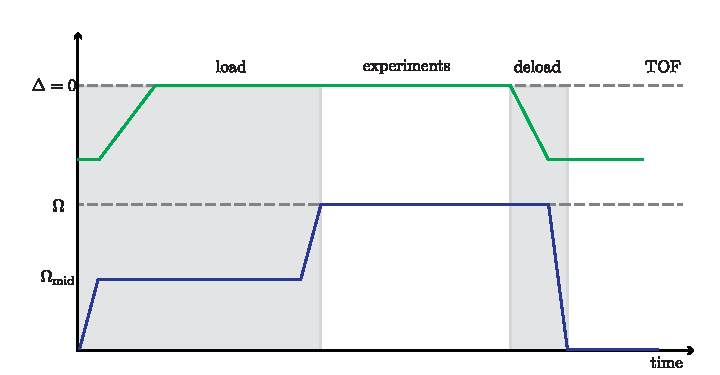
\includegraphics[]{Figures/Chapter6/loading_xyz_traces}
    \caption[Experimental CCD protocol]{Detuning and RF coupling strengths ramps (not to scale) performed to adiabatically prepare the $\xyz$ states starting in the $\ket{m_F}$ states and vice versa.}
    \label{fig:ccd_protocol}
\end{figure*}



\section{Initial characterization of $\Omega$}

Producing RF fields with large coupling strength was not a trivial task and when testing different antenna designs it was important to have an easy and quick way of characterizing them. We mostly relied on two different techniques to get an initial estimate of $\Omega$: first, we prepared atoms in $\ket{m_F=-1}$ and pulse on the RF to drive transitions between the three $\ket{m_F}$ states. We would then fit the populations in the three states as a function of pulsing time to the time evolution given the time dependent Sch\"odinger equation for the RF Hamiltonian (Equation~\ref{eq:h0}) with $\Omega$ and $\Delta$ as free parameters. 

\begin{figure*}[ht]
    \centering
    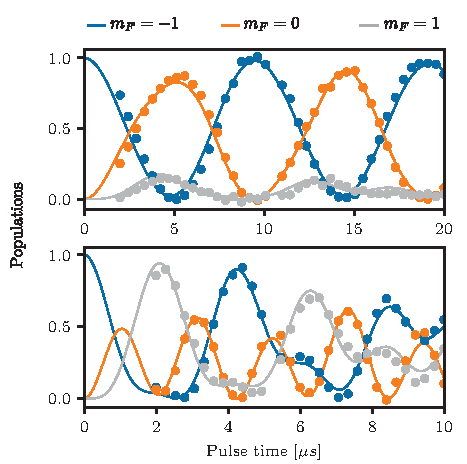
\includegraphics[]{Figures/Chapter6/Rabi_flop_calibrations.pdf}
    \caption[Calibration of $\Omega$]{We prepared the system in the $\ket{m_F=-1}$ state and pulsed $\Omega$ for variable times. We fit the populations in the $\ket{m_F}$ states as a function of pulsing time to get an initial estimate of $\Omega$. The top panel shows the time evolution of $\Omega/2\pi\approx\unit[76]{kHz}$ and the bottom panel shows the evolution for $\Omega/2\pi\approx\unit[238]{kHz}$}
    \label{fig:rabi_calibration}
\end{figure*}

Alternatively, we followed the loading procedure described in Section\ref{sec:xyz_state_preparation} but suddenly turned $\Omega$ off for different values of $\Delta$ to get the decomposition of the $\xyz$ states in terms of the $\ket{m_F}$ states. We then fit the populations to the eigenstates of the Equation~\ref{eq:h0} with $\Omega$ and $\Delta$ as free parameters. Figure~\ref{fig:s1} is an example of such type of calibration. 

For an antenna with a high quality factor such as ours ($q\sim20$) we could not `suddenly' turn $\Omega$ on or off as it takes some time for power to build up and to die out when the RF fields are turned on or off. If we did not include this into the model used to calibrate $\Omega$ we could get some results that were slightly off. We only used these measurements as initial estimates and once we found an antenna design that could produce a large enough $\Omega$ we used the spectroscopy techniques described in the next section to fully characterize the system. 

\section{Spectroscopy}
We confirmed our control and measurement techniques spectroscopically by measuring the energy differences between the $\xyz$ states with an additional probing field with angular frequency $\omega+\omega_p$, coupling strength $\Omega_p$ and polarized along $\ey$. In the frame rotating with angular frequency $\omega$ and after using a RWA the system was described by the Hamiltonian 
%
\begin{align}
    \hat H = \Delta\hat F_z &+ \hbar\epsilon(\hat F_z^2 / \hbar^2 - \hat{\mathbb I}) + \Omega \hat F_x \nonumber \\
    &+ \Omega_p \left(\sin(\omega_p t) \hat F_x + \cos(\omega_p t) \hat F_y\right).
    \label{eq:h}
\end{align}
%
In this rotating frame the probe field initially polarized along $\ey$ has components along $\ex$ and $\ey$, resulting in at least one non-zero transition matrix element for all transitions between pairs of dressed states. If the probing field was polarized along $\ez$ we would not be able to drive the $zy$ transition as can be seen from the matrix elements in Equation~\ref{eq:matrix_elements}.

To probe the dependence of the $\xyz$ state energies on detuning, we performed Rabi spectroscopy (Section~\ref{sec:Rabi_oscillations}) by pulsing $\Omega_p$ on for a constant time and scanned $\omega_p$ for different values of $\Delta$. Figure~\ref{fig:1}b shows the spectroscopically resolved values of $\omega_{xy}/2\pi$, $\omega_{yz}/2\pi$, and $\omega_{zx}/2\pi$ for $\Omega/2\pi=\SI{194.5(1)}{kHz}$ and the side panel shows a sample spectra measured with coupling strength $\Omega_p/2\pi \approx \SI{1}{kHz}$ and $\Delta/2\pi \approx \SI{9}{kHz}$. The dashed curves were computed by diagonalizing \refeq{eq:h0}, and they clearly depart from our measurements for the $zx$ transition.
This departure results from neglecting the weak dependence of the quadratic shift $\epsilon$ on bias field $B_0$. In near-perfect agreement with experiment, the solid curves from the full Breit-Rabi expression account for this dependency.
%
\begin{figure*}[ht]
    \centering
    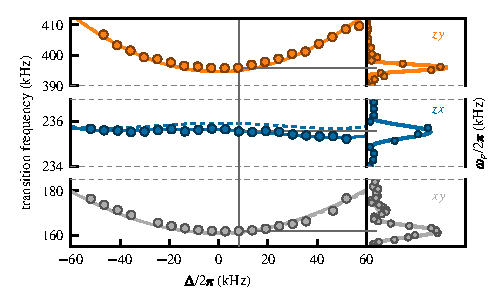
\includegraphics[]{Figures/Chapter6/fig1b}
    \caption[Spectroscopy of the $\xyz$ states]{Left: spectroscopic data showing transitions between the $\xyz$ states for $\Omega/2\pi = \SI{194.5(1)}{kHz}$.
    The vertical scale of the center panel ($zx$ transition) has only $10\%$ the range of the other panels. The dashed lines correspond to the Hamiltonian of \refeq{eq:h0} while the solid lines include the dependence of the quadratic shift on $\Delta$.Right: representative spectra.}
    \label{fig:xyz_spextroscopy}
\end{figure*}
%
\begin{figure}[!!h]
    \centering
    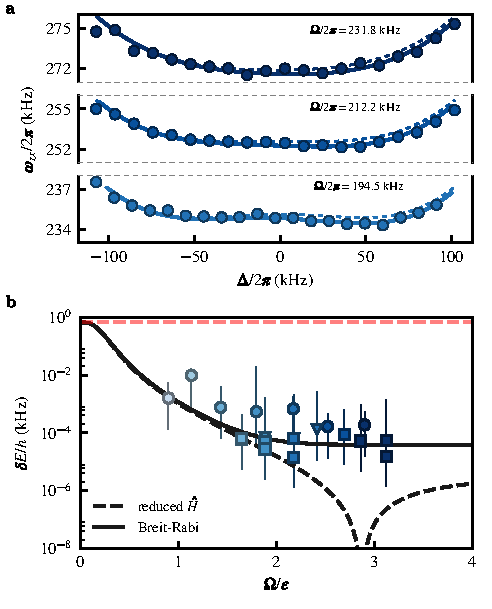
\includegraphics[]{Figures/Chapter6/fig2.pdf}
    \caption[The $\ket{z}\rightarrow\ket{x}$ transition as a function of $\Omega_{\rm RF}$]{{\bf a.} Transition frequency $\omega_{zx}/2\pi$ for three values of $\Omega/2\pi$.
    The dashed curves correspond to \refeq{eq:h}, while the solid curves use the Breit-Rabi expression.
    {\bf b.} The change in energy from our experimental detuning fluctuations as measured in the $\ket{m_F}$ basis is $\delta \Delta/2\pi = \SI{0.67}{kHz}$ (red dashed line).
    Triangles correspond to $\xyz$ spectroscopy data, squares to side-of-peak $\pi$-pulse data, and circles to double-dressed data.
    The black dashed (solid) curve was calculated using \refeq{eq:h} (the Breit-Rabi expression).
    The shading of the data points corresponds to the Rabi frequencies in \reffig{fig:3}.}
    \label{fig:2}
\end{figure}

\section{Robustness}
We focus on the robustness of the $zx$ transition which can be made virtually independent of magnetic field variations due to the similar curvature of $\omega_z(\Delta)$ and $\omega_x(\Delta)$ (see the middle panel of \reffig{fig:1}b). We quantified the sensitivity of this transition to field variations with three methods corresponding to the different markers in \reffig{fig:2}b:
(1) Triangles denote data using Rabi spectroscopy as in \reffig{fig:2}a.
(2) Squares denote data in which a detuned $\pi$-pulse of the probe field transferred approximately half of the atoms from $\ket z$ to $\ket x$. This `side-of-peak' technique overcomes the limitation of Rabi spectroscopy being first-order insensitive to changes in $\omega_{zx}$.
(3) Circles describe data using a double dressing technique that will be described in Section~\ref{sec:concatenated_cdd}.
In each case we measured the energy shift from resonance as a function of detuning (magnetic field) and then used a fourth-order polynomial fit to extract the RMS residuals $\delta \omega_{zx}$ due to the known detuning noise~\footnote{Our procedure also quantifies the small fluctuations that survive for spectra that are flat beyond second order, as in \refeq{eq:h0}.}. The results are not consistent with the theory simple from \refeq{eq:h} (dashed) and instead require the Breit-Rabi expression (solid) to obtain full agreement~\footnote{The fluctuations can be even smaller for a given $\Omega$ if we allow for $\Delta \neq 0$.}.

Even at our smallest coupling $\Omega/2\pi=\SI{69(1)}{kHz}$ the typical magnetic field noise was attenuated by two orders of magnitude, rendering it essentially undetectable. Ideally, the radius of curvature of $\omega_{zx}(\Delta)$ changes sign at about $\Omega/2\pi = \SI{220}{kHz}$, leaving only a $\Delta^4$ contribution, however, in practice the small dependence of $\epsilon$ on $B$ prevents this perfect cancellation. Still it is possible to see the changing curvature of $\omega_{zx}(\Delta)$ near $\Delta=0$ for different values of $\Omega$ in Figure~\ref{fig:2}a.

\subsection{Optimal response to noise}

The sensitivity of the $zx$ transition to detuning fluctuations can be optimized further by working at $\Delta \neq 0$ as shown in \reffig{fig:sopt}.
%This behavior can only be captured by including the dependence of the quadratic shift on $\Delta$ as given by the Breit-Rabi expression.

For small values of $\Omega$, the optimum value of $\Delta$ corresponds to one of the concave features of the $zx$ transition energy that arises due to the asymmetry introduced by the quadratic shift.
As $\Omega$ gets larger, these features merge into a single one and the optimum value is $\Delta \approx 0$.
The deviation from $\Delta=0$ is due to an overall tilt of the transition energy coming from the dependence of the quadratic shift on $\Delta$.
At the optimum point $\Omega/\epsilon \approx 3$ the sensitivity of the synthetic clock transition is \SI{1.9e-07}{kHz}, c.f, the $\Rb87$ clock transition which scales as \SI{57.5}{kHz/mT^2} and gives \SI{5.8e-07}{kHz}.
\begin{figure*}[ht]
    \centering
    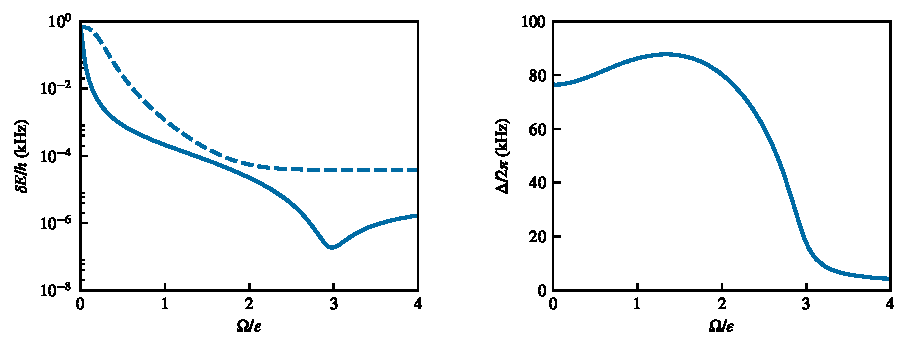
\includegraphics[]{Figures/Chapter6/figS13}
    \caption[Optimal response of the $zx$ transition]{Left: Optimum response (solid) of the $zx$ transition to detuning fluctuations allowing for finite $\Delta$ compared to $\Delta=0$ (dashed) for the full Breit-Rabi model.
    Right: The values of $\Delta$ that correspond to the minimum derivative of $\omega_{zx}$.}
    \label{fig:sopt}
\end{figure*}

\section{Driving dressed state transitions}
\begin{figure}[ht]
    \centering
    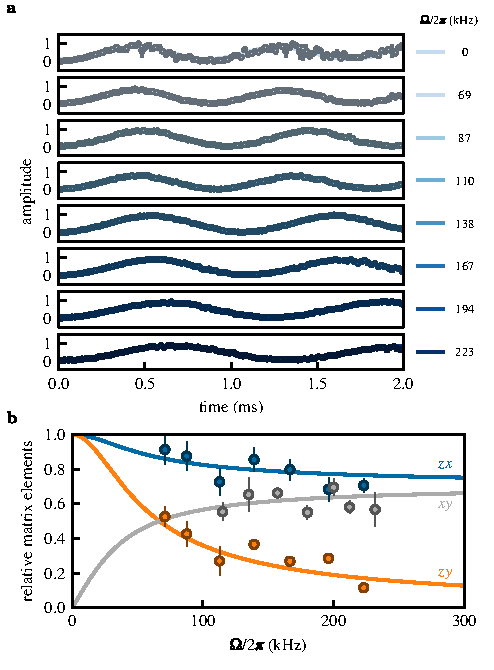
\includegraphics[]{Figures/Chapter6/fig3.pdf}
    \caption[Coherent driving of dressed state transitions]{{\bf a.} Rabi oscillations.
    Phase coherence is maintained throughout the oscillations in the dressed basis, while it is quickly lost in the $\ket{m_F}$ basis.
    The marker size reflects the typical uncertainties on the dressed basis oscillations.
    {\bf b.} Transition matrix elements for $zx$ (blue) and $zy$ (orange) transitions decrease monotonically with increasing $\Omega$ for $\Delta=0$, while they increase for $xy$.
    }
    \label{fig:3}
\end{figure}
We explored the strength of the probe-driven transitions between these states by observing coherent Rabi oscillations (\reffig{fig:3}a) where our BEC was prepared in $\ket z$ and the probe field had strength $\Omega_p/2\pi\approx\SI{1}{kHz}$.
The top panel shows Rabi oscillations between $\ket{m_F=0}$ and $\ket{m_F=-1}$ states for reference, and the remaining panels show oscillations between $\ket{z}$ and $\ket{x}$.
The observed Rabi frequency between dressed states decreased with increasing $\Omega$ indicating a dependence of the $zx$ transition matrix elements on $\Omega$. We repeated this experiment driving all possible pairs of dressed state transitions at fixed $\Omega_p$ for,  and \reffig{fig:3}b shows the dependence of these matrix elements on $\Omega$ for $\Delta=0$.

The coherence of the Rabi oscillations for longer times was limited by gradients in $\Omega$ that lead to phase separation of the dressed states, and therefore loss of contrast in the oscillations. This effect was faster for smaller frequency Rabi oscillations. For example for $\Omega_p/2\pi=\unit[5]{kHz}$ we observed coherent Rabi oscillations with almost full contrast for more than $\unit[10]{ms}$ while for the $\Omega_p/2\pi=\unit[870]{Hz}$ oscillation shown in Figure~\ref{fig:decaying_rabi} the contrast was significantly reduced after $\unit[5]{ms}$. The loss of contrast was even worse when we tried performing a Ramsey sequence where the time evolution is most sensitive to the environment. One solution to this problem would be to change the experimental setup to a double loop antenna to generate a more spatially uniform magnetic field. 
%
\begin{figure}[ht]
    \centering
    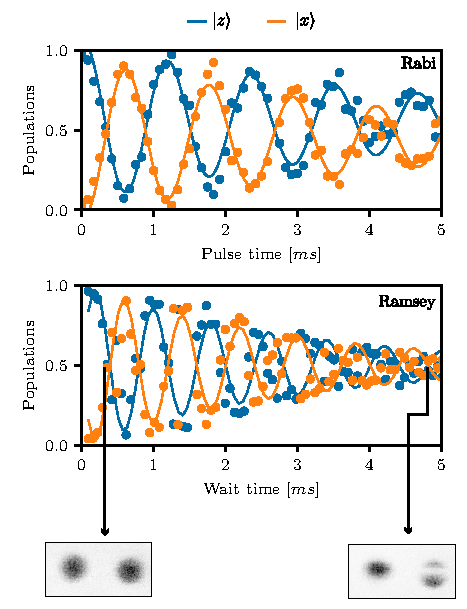
\includegraphics[]{Figures/Chapter6/RF_Ramsey.pdf}
    \caption[Loss of contrast of coherent oscillations]{Loss of contrast in coherent oscillations. A Rabi oscillation (top) between the $\ket{z}$ and $\ket{x}$ states with $\Omega_p/2\pi=\unit[870]{Hz}$ decays by $1/e$ in $\unit[4.6]{ms}$ and a Ramsey oscillation (middle) with about $\unit[1]{kHz}$ frequency decays in about $\unit[3]{ms}$. The gradients in $\Omega$ lead to phase separation of dressed states and loss of contrast for longer pulse/wait times.  
    }
    \label{fig:decaying_rabi}
\end{figure}

In comparison, we found that for both Rabi and Ramsey oscillations between the $\ket{m_F}$ states the phase started deteriorating after a few hundreds of $\us$, this is not surprising due to bias magnetic field temporal noise. We canceled gradient magnetic fields so that no phase separation of the bare states was observed for $>\SI{10}{sec}$. As a result, the system can in principle undergo coherent evolution without loss of contrast for a long time but because of field fluctuations between shots what we observed instead was full contrast noise. 

\section{Concatenated CDD }
\label{sec:concatenated_cdd}
The driving field $\Omega$ coupled together the $\ket{m_F}$ states, giving us the $\xyz$ synthetic clock states that were first-order insensitive to magnetic field fluctuations. However, the spectrum of these states is still first-order sensitive to fluctuations of the driving field $\delta \Omega$. Reference~\cite{cai_robust_2012} showed that an additional field coupling together with these $\xyz$ states can produce doubly-dressed states that are insensitive to both $\delta \Omega$ and $\delta \Delta$: a process called concatenated CDD.
In our experiment, the probe field provided the concatenating coupling field. 
Because $\Omega_p\ll\Omega$, we focus on a near-resonant two-level system formed by a single pair of dressed states, here $\ket{z}$ and $\ket{x}$, which we consider as pseudospins $\ket{\!\uparrow}$ and $\ket{\!\downarrow}$.
These states are described by the effective two-level Hamiltonian
\begin{equation}
    \hat H_p = \frac{\hbar\Delta'}{2} \hat \sigma_3 + \hbar\Omega' \cos(\omega_p t) \hat \sigma_1,
    \label{eq:h2}
\end{equation}
with energy gap $\Delta' \approx \omega_{z,x}$ (shifted by off-resonant coupling to the $zy$ and $xy$ transitions) and coupling strength $\Omega' \propto \Omega_p$, as set by the matrix elements displayed in~\reffig{fig:3}b.
Here $\hat \sigma_{1,2,3}$ are the three Pauli operators.

We perform a second transformation into a frame rotating with angular frequency $\omega_p$ and use a RWA to compute the eigenenergies of Equation~\ref{eq:h2}. For large values of $\Omega'$ the energies take the values $E_{\uparrow,\downarrow} \approx \pm\Omega^\prime/2 + (\Delta^\prime)^2/2\Omega^\prime$. Even though $E_{\uparrow,\downarrow}$ are still first order sensitive to $\Omega$ because $\Delta'\approx\omega_{z,x}\propto\Omega$, its effect is suppressed by a factor of $1/\Omega'$. Thus, the concatenated CDD field protects from the fluctuations $\delta\Delta^{\prime}$ of the first dressing field in a similar way that CDD provided protection from detuning noise $\delta \Delta$. Table~\ref{table:CDD} summarizes the dependence of the $\xyz$ and $\ket{\uparrow\downarrow}$ energies on $\Delta$, $\Omega$ and $\Omega'$. 
%
\begin{table}[h]
\caption[Summary of CDD energies]{Energies of the CDD and CCDD states as a function of $\Delta$, $\Omega$ and $\Omega'$. The dependence on parameters not relevant to the expansion is given by the functions $f_1$, $f_2$, $g_1$ and $g_2$.}
\begin{center}
\begin{tabular}{c|c|c}
\hline
 % & & \\
 & CDD & concatenated CDD \\
 % & & \\
\hline \hline
 % & & \\
$\Delta$ dependence  & $f_1(\epsilon,\Omega)\Delta^2$ & $f_2(\Omega,\epsilon)\frac{\Delta^2}{\Omega'}$ \\
 & & \\
\hline
 % & & \\
$\Omega$, $\Omega'$ dependence & $\Omega+g_1(\Delta, \epsilon)\frac{1}{\Omega}$ &  $\left[\Omega^2 + \epsilon\Omega + g_2(\Delta, \epsilon)\frac{1}{\Omega}\right]\frac{1}{\Omega'}$ \\
 & & \\  
% \hline
\end{tabular}
\end{center}
\label{table:CDD}
\end{table}

We produced doubly-dressed states by doing (one more!) ARP sequence. We initialized the system in the $\ket{\!\downarrow}$ state with RF coupling strength $\Omega_i$. We set the probe frequency to be $\sim\unit[20]{kHz}$ off resonant with respect to the $\ket{\, \downarrow}\rightarrow \ket{\, \uparrow}$ transition and ramped it on in $\unit[10]{ms}$. We then ramped $\Omega_i\rightarrow\Omega_f$ in $\unit[30]{ms}$. The experimental sequence can be visualized in Figure~\ref{fig:concatenated_cdd}. We chose the value of $\Omega_f$ such that it would bring $\omega_p$ to resonance at $\Delta=0$, creating double dressed states that were equal superposition of $\ket{\,\downarrow}$ and $\ket{\,\uparrow}$. We quantified the sensitivity of this transition to large changes in the detuning $\Delta$ in terms of the fractional population imbalance $\langle\hat\sigma_3\rangle = P_\downarrow(\Delta)-P_\uparrow(\Delta)$, shown in \reffig{fig:4}a for $\Omega_f/2\pi=\SI{138.2(1)}{kHz}$~\footnote{We chose the maximum value of $\Delta$ such that the population of \unexpanded{$\ket y$}, was negligible after deloading.}.
This signal is first-order sensitive to $\omega_{\downarrow, \uparrow}$, and provided our third measurement of sensitivity to detuning in \reffig{fig:2}b denoted by circles.
\begin{figure}[!ht]
    \centering
    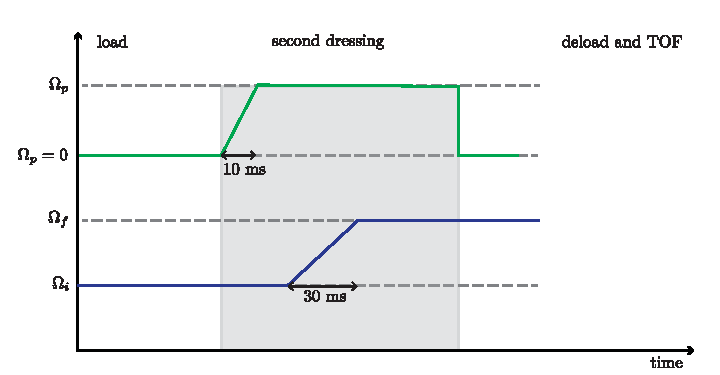
\includegraphics[]{Figures/Chapter6/concatenated_cdd.pdf}
    \caption[Concatenated CDD protocol]{Experimental protocol for implementing concatenated CDD. We started an initial RF coupling strength $\Omega_i$ and ramped on the probe field $\Omega_p$ in a few ms with $\omega_p=\omega_{z,x}(\Omega_f)$ so that it was initially slightly off resonant with the $zx$ transition. We then ramped the RF field to $\Omega_f$, brining $\omega_p$ to resonance. 
    }
    \label{fig:concatenated_cdd}
\end{figure}
\begin{figure}[h]
    \centering
    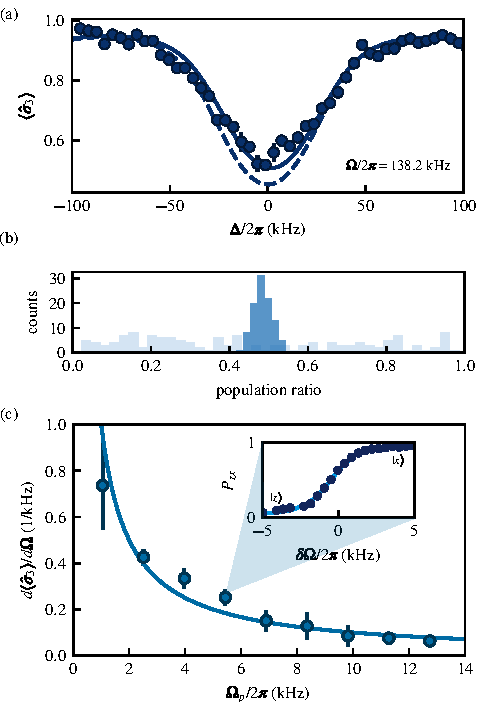
\includegraphics[]{Figures/Chapter6/fig4.pdf}
    \caption[Concatenated CCD]{(a) The fractional population imbalance of the $\downarrow\uparrow$ transition for $\Omega/2\pi=\SI{138.2(1)}{kHz}$ over detuning $\Delta$.
    The dashed curve is calculated using \refeq{eq:h} and the solid one using the full Breit-Rabi expression.
    (b) The fidelity of preparing a balanced superposition of $\ket{\!\downarrow}$ and $\ket{\!\uparrow}$ (dark blue) states compared to $\ket{m_F=0}$ and $\ket{m_F=-1}$ states (light blue).
    (c) The robustness of $\downarrow, \uparrow$ transition against fluctuations $\delta \Omega$ for different probe field coupling strengths.
    The points represent the slope of the fitted curves to the fractional population imbalance (inset).}
    \label{fig:4}
\end{figure}

We compared the fidelity of preparing a superposition of the $\ket{\,\downarrow}$ and $\ket{\,\uparrow}$ states to adiabatically preparing a similar superposition of the the $\ket{m_F=0}$ and $\ket{m_F=-1}$ states using a single ARP (no dressed states involved), both with a probe field strength of  $\approx\SI{1}{kHz}$.
Figure~\ref{fig:4}b shows the RMS deviation of the population imbalance measured over a few hundred repetitions of the experiment.
The RMS deviation for the dressed basis is $0.024(1)$ and is an order of magnitude smaller than for the $\ket{m_F}$ basis $0.29(1)$, where it practically impossible to prepare a balanced superposition for the parameters used here~\footnote{In \reffig{fig:4}b, the noise in the $\ket{m_F}$ basis is not Gaussian distributed as is typical of line noise in these experiments.}.

Figure~\ref{fig:4}c shows the response of the $\ket{\, \downarrow}\rightarrow \ket{\, \uparrow}$ transition to small changes $\delta\Omega$ for different values of $\Omega_p$.
We prepared an equal superposition of $\ket{\,\downarrow}$ and $\ket{\,\uparrow}$ following the same procedure as before for $\Omega_f/2\pi = \SI{138.2(1)}{kHz}$.
We then measured how the population imbalance changes for small variations of $\Omega$ --- the effective detuning in the `twice-rotated frame' --- for different probe amplitudes $\Omega_p$.
We defined a sensitivity parameter $d\langle\hat\sigma_3\rangle / d\Omega$, obtained from the linear regime of the population imbalance measurements (see inset in \reffig{fig:4}c).
The robustness of the doubly-dressed states against $\delta \Omega$ fluctuations increased with $\Omega_p$, thus verifying the concatenating effect of CDD in the $\xyz$ basis.

However promising the application of multiple concatenating fields might seem, this procedure has a fundamental limitation. Each time a new coupling field is applied the energies of the dressed states are reduced to something on the order of magnitude of the coupling strength from the applied concatenating field. For example, in the experiments we described here we started with $\ket{m_F}$ states with transition frequencies on the order of MHz. The transition frequencies of the $\ket{xyz}$ states were reduced to hundreds of kHz (or in general the magnitude of $\Omega$). After applying the second concatenating RF field the transition frequencies of the $\ket{\!\downarrow\uparrow}$ are of the order of $\Omega_p\sim\unit[10]{kHz}$ which needs to be smaller than $\Omega$ for the second RWA to be valid. Therefore we see that after applying multiple concatenating fields we are at the risk of having some very robust states that are also very closely spaced in energy which might not be desirable for some applications. 

\section{Conclusions}
We realized a three-level system that is dynamically decoupled from low-frequency noise in magnetic fields, measured now-allowed transitions between all three states, and demonstrated control techniques for creating arbitrary Hamiltonians.  These techniques add no heating or loss mechanisms, yet within the protected subspace retain the full complement of cold-atom coherent control tools such as optical lattices and Raman laser coupling, and permit new first-order transitions that are absent in the unprotected subspace.
These transitions enable experiments requiring a fully connected geometry as for engineering exotic states, e.g., in cold-atom topological insulators, and two-dimensional Rashba spin-orbit coupling in ultracold atomic systems~\cite{campbell_rashba_2016, juzeliunas_generalized_2010}.

The synthetic clock states form a decoherence-free subspace that can be used in quantum information tasks where conventional clock states might be absent, or incompatible with other technical requirements~\cite{bacon_universal_2000}.
Moreover, their energy differences are proportional to the amplitude of the dressing field, and hence tunable, so they can be brought to resonance with a separate quantum system.
The effective quantization axis can be arbitrarily rotated so that the two systems can be strongly coupled, pointing to applications in hybrid quantum systems~\cite{solano_chapter_2017,xiang_hybrid_2013}.
Introducing a second coupling field shields the system from fluctuations of the first, a process that can be concatenated as needed.
More broadly, synthetic clock states should prove generally useful in any situation where fluctuations of the coupling field can be made smaller than those of the environment.

% \section{Locating field resonance}

% We used an iterative procedure to measure and adjust the value of the detuning $\Delta$ to account for the weak response of the $\xyz$ states to detuning variations.
% As most of our experiments were done at $\Delta=0$, we first obtained an estimate of $\Delta$ from the imbalance of $\ket 1$ and $\ket{-1}$ populations from the decomposition of $\ket z$ which should be zero for $\Delta=0$ (see \reffig{fig:s1}).
% We then located the transition frequencies for at least two transitions (usually $zx$ and $zy$ as shown in \reffig{fig:s2}) using an ARP protocol as described in the main text and varying the frequency of the probe field.
% These frequencies correspond to a unique pair of $\Omega$ and $\vert\Delta\vert$ values which can then be used to adjust the bias magnetic field $B_0$ so that $\Delta=0$.
% However, there is an ambiguity as to the sign of $\Delta$ since the eigenstates are even functions of $\Delta$.

% We selected a direction randomly and subsequently verified if $\Delta=0$ using another set of spectroscopic measurement.
% We fixed the value of the probe field to be a few kHz above the transition frequency corresponding to $\Delta=0$ and used the same ARP sequence to transfer atoms from $\ket z$ to $\ket x$.
% This procedure gave two resonant values for $\Delta$ were atom transfer takes place, and the value where $\Delta=0$ corresponded to their mean (see \reffig{fig:s2}).
% Finally, we remeasured the $zx$ and $zy$ transition frequencies to validate that $\Delta=0$.
% For higher values of $\Omega_R$, using the $zx$ transition becomes impractical
% due to its insensitivity to detuning, and we followed the same procedure but using the $xy$ transition instead.









